%!TEX TS-program = pdflatex
%!TEX root = tesi.tex
%!TEX encoding = UTF-8 Unicode

\chapter{Introduction}

With the spread of the Internet and more importantly of the social networks, efficient data analysis on graphs becomes increasingly important.
Graphs are a powerful data structure that natural model the interactions between objects.

%%%%%%%%%%%%%%%%%%%%%%%%%%%%%%%%%%%%%%%%%%%%%%%%%%%%%%%%%%%%%%%%%%%%%%%%%%%%%%%%%%%%%%%%%%%%%%
%%%%%%%%%%%%%%%%%%%%%%%%%%%%%%%%%%%%%%%%%%%%%%%%%%%%%%%%%%%%%%%%%%%%%%%%%%%%%%%%%%%%%%%%%%%%%%

\section{Basic definitions}

\begin{definizione}\label{def:graph}
    A \textbf{graph} is a pair of sets $G=(V,E)$, where $V$ is the set of vertices (or nodes) and $E \subset V \times V$ is the set of edges.
\end{definizione}

If two vertices $u, v \in V$ are connected by an edge they are called extreme of the edge, in this case we denote the edge with the pair $(u, v) \in E$

If $(u,v) \in E \Leftrightarrow (v,u) \in E$ the graph is called undirected, where not specified we will only deal with undirected graphs.

A sequence of nodes  $v_{1}, v_{2}, \ldots, v_{k}$ is called path if $(v_{i}, v_{i+1}) \in E$ $\forall i = 1, \ldots k-1$; a path is called simple if $v_{i} \neq v_{j}$ $\forall i,j$ $1 \leq i < j \leq k$. A cycle is a path where $(v_{k}, v_{1}) \in E$.

We denote by $N(u) = \{ v : (u,v) \in E \}$ the set of neighbors of the vertex $u$, the cardinality of this set is called degree of $u$ (\textit{deg} $u$ = $|N(u)|)$. 

With $N^{<k}(u)$ we indicate the set of vertex connected to $u$ by a simple path of length less than $k$ (note that $N(u)$ = $N^{<2}(u)$).

\begin{definizione}\label{def:subgraph}
    A graph $G' = (V', E')$ is called \textbf{subgraph} of $G=(V,E)$ if $V' \subset V$ and $E' \subset E$. A subgraph is called \textbf{induced subgraph} if $E' = (V' \times V') \cap E$.
\end{definizione}

We use $G' \subset G$ to indicate that the graph $G'$ is a subgraph of $G$ and $G' < G$ to indicate that the graph $G'$ is a induced subgraph of $G$.\\

Note that an induced subgraph $G' = (V', E')$ can be uniquely identified by the set of its vertex $V'$.

\begin{definizione}\label{def:labeledgraph}
	A \textbf{labeled graph} is a triple $(V,E,L)$ where $(V,E)$ is a graph and $L : V \rightarrow \Sigma$
	is a function that assign for every node $v$ a symbol of the alphabet $\Sigma$. We call $L(u) \in \Sigma$ label of the node $u$.
\end{definizione}

Given a path $\pi = v_{1}, v_{2}, \ldots, v_{k}$ we extend the function $L$ and we indicate with $L(\pi) = L(v_{1}) L(v_{2}) \ldots L(v_{k}) \in \Sigma^{k}$ the string obtained by the concatenation of the labels of the nodes in the path.\\

In this thesis we mainly focus to analyze complex network: special graphs with a non-trivial topology like random graphs. Complex network occur in graphs modeling real system like social networks or computer networks and are characterized by a specific structural feature:

\begin{definizione}\label{def:power-law-graph}
	We define as \textbf{power-law degree distribution} a networks where the degree of a node $u$ follow, for some $\gamma$ (usually $2 < \gamma < 3$), the probability distribution:
	\begin{equation}
		P(deg(u) = k) \sim k^{-\gamma}  
	\end{equation}
\end{definizione}

\begin{figure}[h]
	\centering
	\begin{minipage}[t]{.45\textwidth}
		\centering
		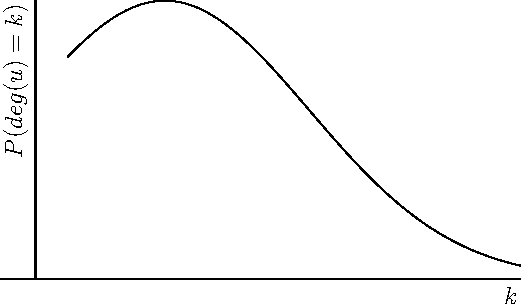
\includegraphics[width=5cm,height=3cm]{figure/figure-1-1}
		\caption{Degree distribution of a random network}
	\end{minipage}\hfill
	\begin{minipage}[t]{.45\textwidth}
		\centering 
		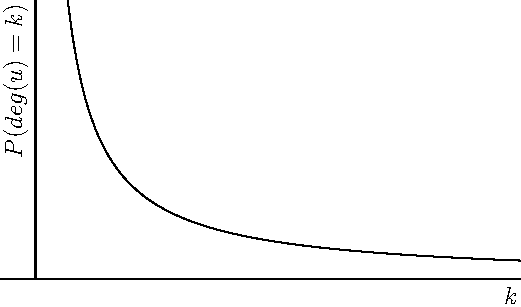
\includegraphics[width=5cm,height=3cm]{figure/figure-1-2}
		\caption{Degree distribution of a complex network}
	\end{minipage}
\end{figure}

\begin{figure}[h]
	\centering
	\begin{minipage}[t]{.45\textwidth}
		\centering
		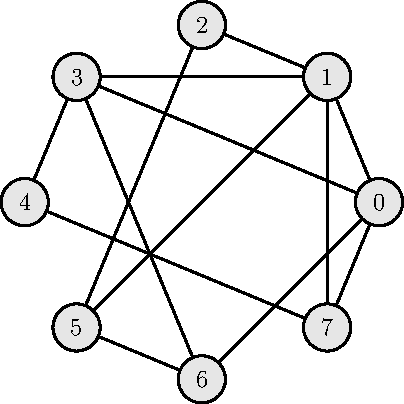
\includegraphics[width=3cm,height=3cm]{figure/figure-1-3}
		\caption{Random network}
	\end{minipage}\hfill
	\begin{minipage}[t]{.45\textwidth}
		\centering
		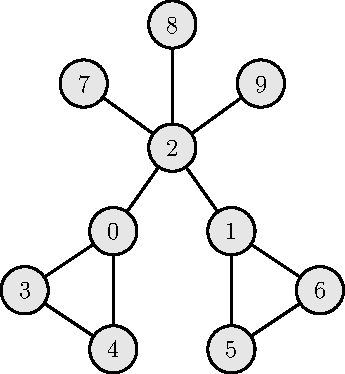
\includegraphics[width=2.8cm,height=3cm]{figure/figure-1-4}
		\caption{Complex network}
	\end{minipage}
\end{figure}

\clearpage
%%%%%%%%%%%%%%%%%%%%%%%%%%%%%%%%%%%%%%%%%%%%%%%%%%%%%%%%%%%%%%%%%%%%%%%%%%%%%%%%%%%%%%%%%%%%%%
%%%%%%%%%%%%%%%%%%%%%%%%%%%%%%%%%%%%%%%%%%%%%%%%%%%%%%%%%%%%%%%%%%%%%%%%%%%%%%%%%%%%%%%%%%%%%%
\section{The problem}

\begin{problema}
Given an undirected labeled graph $G=(V,E,L)$ over an alphabet $\Sigma$, an integer $q$
and two set of nodes $V_{1}, V_{2} \subset V$, we want to estimate the similarity between the two induced subgraphs $V_{1}, V_{2} < G$ based on the labels frequency of simple paths with nodes in $V_{1} \cup N^{<q}(V_{1})$ and $V_{2} \cup N^{<q}(V_{2})$.
\end{problema}

We will talk about a more formal and rigorous definition of subgraphs similarity in chapter 2.\\

In the definition we use $V_{1} \cup N^{<q}(V_{1})$ and $V_{2} \cup N^{<q}(V_{2})$ instead of simply $V_{1}$ and $V_{2}$ because, in a complex graph, we also want to keep in mind of the interaction between the subgraph and the external graph.\\

The difficulty we must face is that, in a complex network, the labels can exponentially explode for increasing values of q and $|\Sigma|$ to $|\Sigma|^{q} \gg |V|$ and, even worse, the number of simple paths can exponentially explode to $|V|^{q}$. For the simple reason that in complex networks the average separation is very low (the famous idea of \textit{six degrees of separation}).\\

In this thesis we exploit the problem using randomized techniques and parallelization, which makes the problem suitable even for big networks. 
%%%%%%%%%%%%%%%%%%%%%%%%%%%%%%%%%%%%%%%%%%%%%%%%%%%%%%%%%%%%%%%%%%%%%%%%%%%%%%%%%%%%%%%%%%%%%%
%%%%%%%%%%%%%%%%%%%%%%%%%%%%%%%%%%%%%%%%%%%%%%%%%%%%%%%%%%%%%%%%%%%%%%%%%%%%%%%%%%%%%%%%%%%%%%

\section{Practical applications}

The problem presented can be applied to a lot of contexts. 
We illustrate some examples of practical application by referring to famous websites,
in order to better understand.
In all the examples we assume to work on a \textit{friendship graph} where the nodes are the registered users and 
the edges are the friendship relations between two users.

\paragraph*{Netflix} In order to produce and translate the right television series, we want to estimate the similarity between two geographical groups of viewers, where each viewer is labeled with its favorite film genre.
  
\paragraph*{Amazon} In order to improve advertising campaigns, we want to estimate the similarity between two sets of clients of the same age group, where each client is labeled with the category of objects he buys more frequently.

\paragraph*{Facebook} In order to suggest new friends, we want to estimate the similarity between two users, where each user is labeled with its favorite musical genres.  

% The problem can be applied to a lot of context.
% That is why it is very important to choose the right domains for the values of the $V, E, L, \Sigma, q$:
% \begin{itemize}
% \item $V$ are out object we want to modeling.
% \item $E$ represent the set of interactions, two vertices are connected if exists a relation among them.
% \item $L$ and $\Sigma$ are the category that partition $V$, $|\Sigma|$ should not be too high or to low, note that if $|\Sigma| = 1$ the labeling is useless as $V$ is not really partitioned.
% \item $q$ should be low as $N^{<q}(u)$ could be a large portion of $G$, (e.g. in Facebook for $q \simeq 4$ we have $N^{<q}(u) \simeq G$)\cite{Facebook}.
% \end{itemize}

% Furthermore, we have to choose $G1$ and $G2$ in a way that similarity between two groups answer use some real question, like compare to each other two ego networks or two connected components.\\

% A pratical example: given a social network of people connected by friendship relation, where every people are labeled with their favorite musical genre, estimate the similary, in terms of musical tastes, of two different geographic regions.

\section{Thesis organization}

The thesis is divided in five chapters and one appendix,
the topics covered are respectively:

\begin{itemize}
	\item Chapter 1: \textbf{Introduction}, this chapter, were we have presented some basic definitions in order to introduce the problem we are analyzing.
	
	\item Chapter 2: \textbf{Basic tools}, definition of some similarity indices already existing in the literature and presentation two methods we will use.
	
	\item Chapter 3: \textbf{Computation of subgraph similarity}, presentation of different approaches to compute the subgraph similarity.
	
	\item Chapter 4: \textbf{Project development}, implementation choices and steps of the project development with some experimental results.
	
	\item Chapter 5: \textbf{Conclusion and future works}, conclusions from theoretical and practical analysis of the , with some hypothesis of future works.
	
	\item Appendix A: \textbf{Code snippets}, some important code snippets of the project used for the experimental results.
\end{itemize}

The results in this thesis are joint work with Alessio Conte, Roberto Grossi, Andrea Marino, Kunihiko Sadakane and Takeaki Uno~\cite{SubSim}.